%Every piece of package I've acumulated over the last years
%%%%%%%%%%%%%%%%%%%%%%%%%%%%%%%%%%%%%%%%%%%%%%%%%%%%%%%%%%%%%%%%%%%%%%%%%%%%%%%%%%%%%%%%%%%%%%
\documentclass[a4paper,12pt]{article}
\usepackage[utf8]{inputenc}
\usepackage{imakeidx}
\usepackage{graphicx}
\usepackage{float}
\usepackage{amssymb}
\usepackage{amsmath}
\usepackage[backend=bibtex,style=verbose]{biblatex}
\bibliography{bibliography}
\usepackage{csquotes}
\usepackage{tcolorbox}
\usepackage{multirow}
\usepackage{caption}
\usepackage{afterpage}
\usepackage[margin=1in]{geometry}
\usepackage[english,spanish]{babel}
\usepackage{tikz}
\usepackage{mwe}
\usepackage{circuitikz}
\usepackage{subcaption}
%%%%%%%%%%%%%%%%%%%%%%%%%%%%%%%%%%%%%%%%%%%%%%%%%%%%%%%%%%%%%%%%%%%%%%%%%%%%%%%%%%%%%%%%%%%%%%
\begin{document}
\title{Evaluación Continua de Mecánica II\\ Temas 2-3}
\author{Gabriel D'Andrade Furlanetto}
\maketitle 

\section{Péndulo de Foucault}

\subsection*{a) Escribe la segunda ley de Newton para el grave y demuestra que la tensión $\boldsymbol{T}$ se puede aproximar como $T \approx m\boldsymbol{g}_{ef}$, donde $\boldsymbol{g}_{ef}$ es la gravedad efectiva.}

\begin{figure}[H]
  \centering
  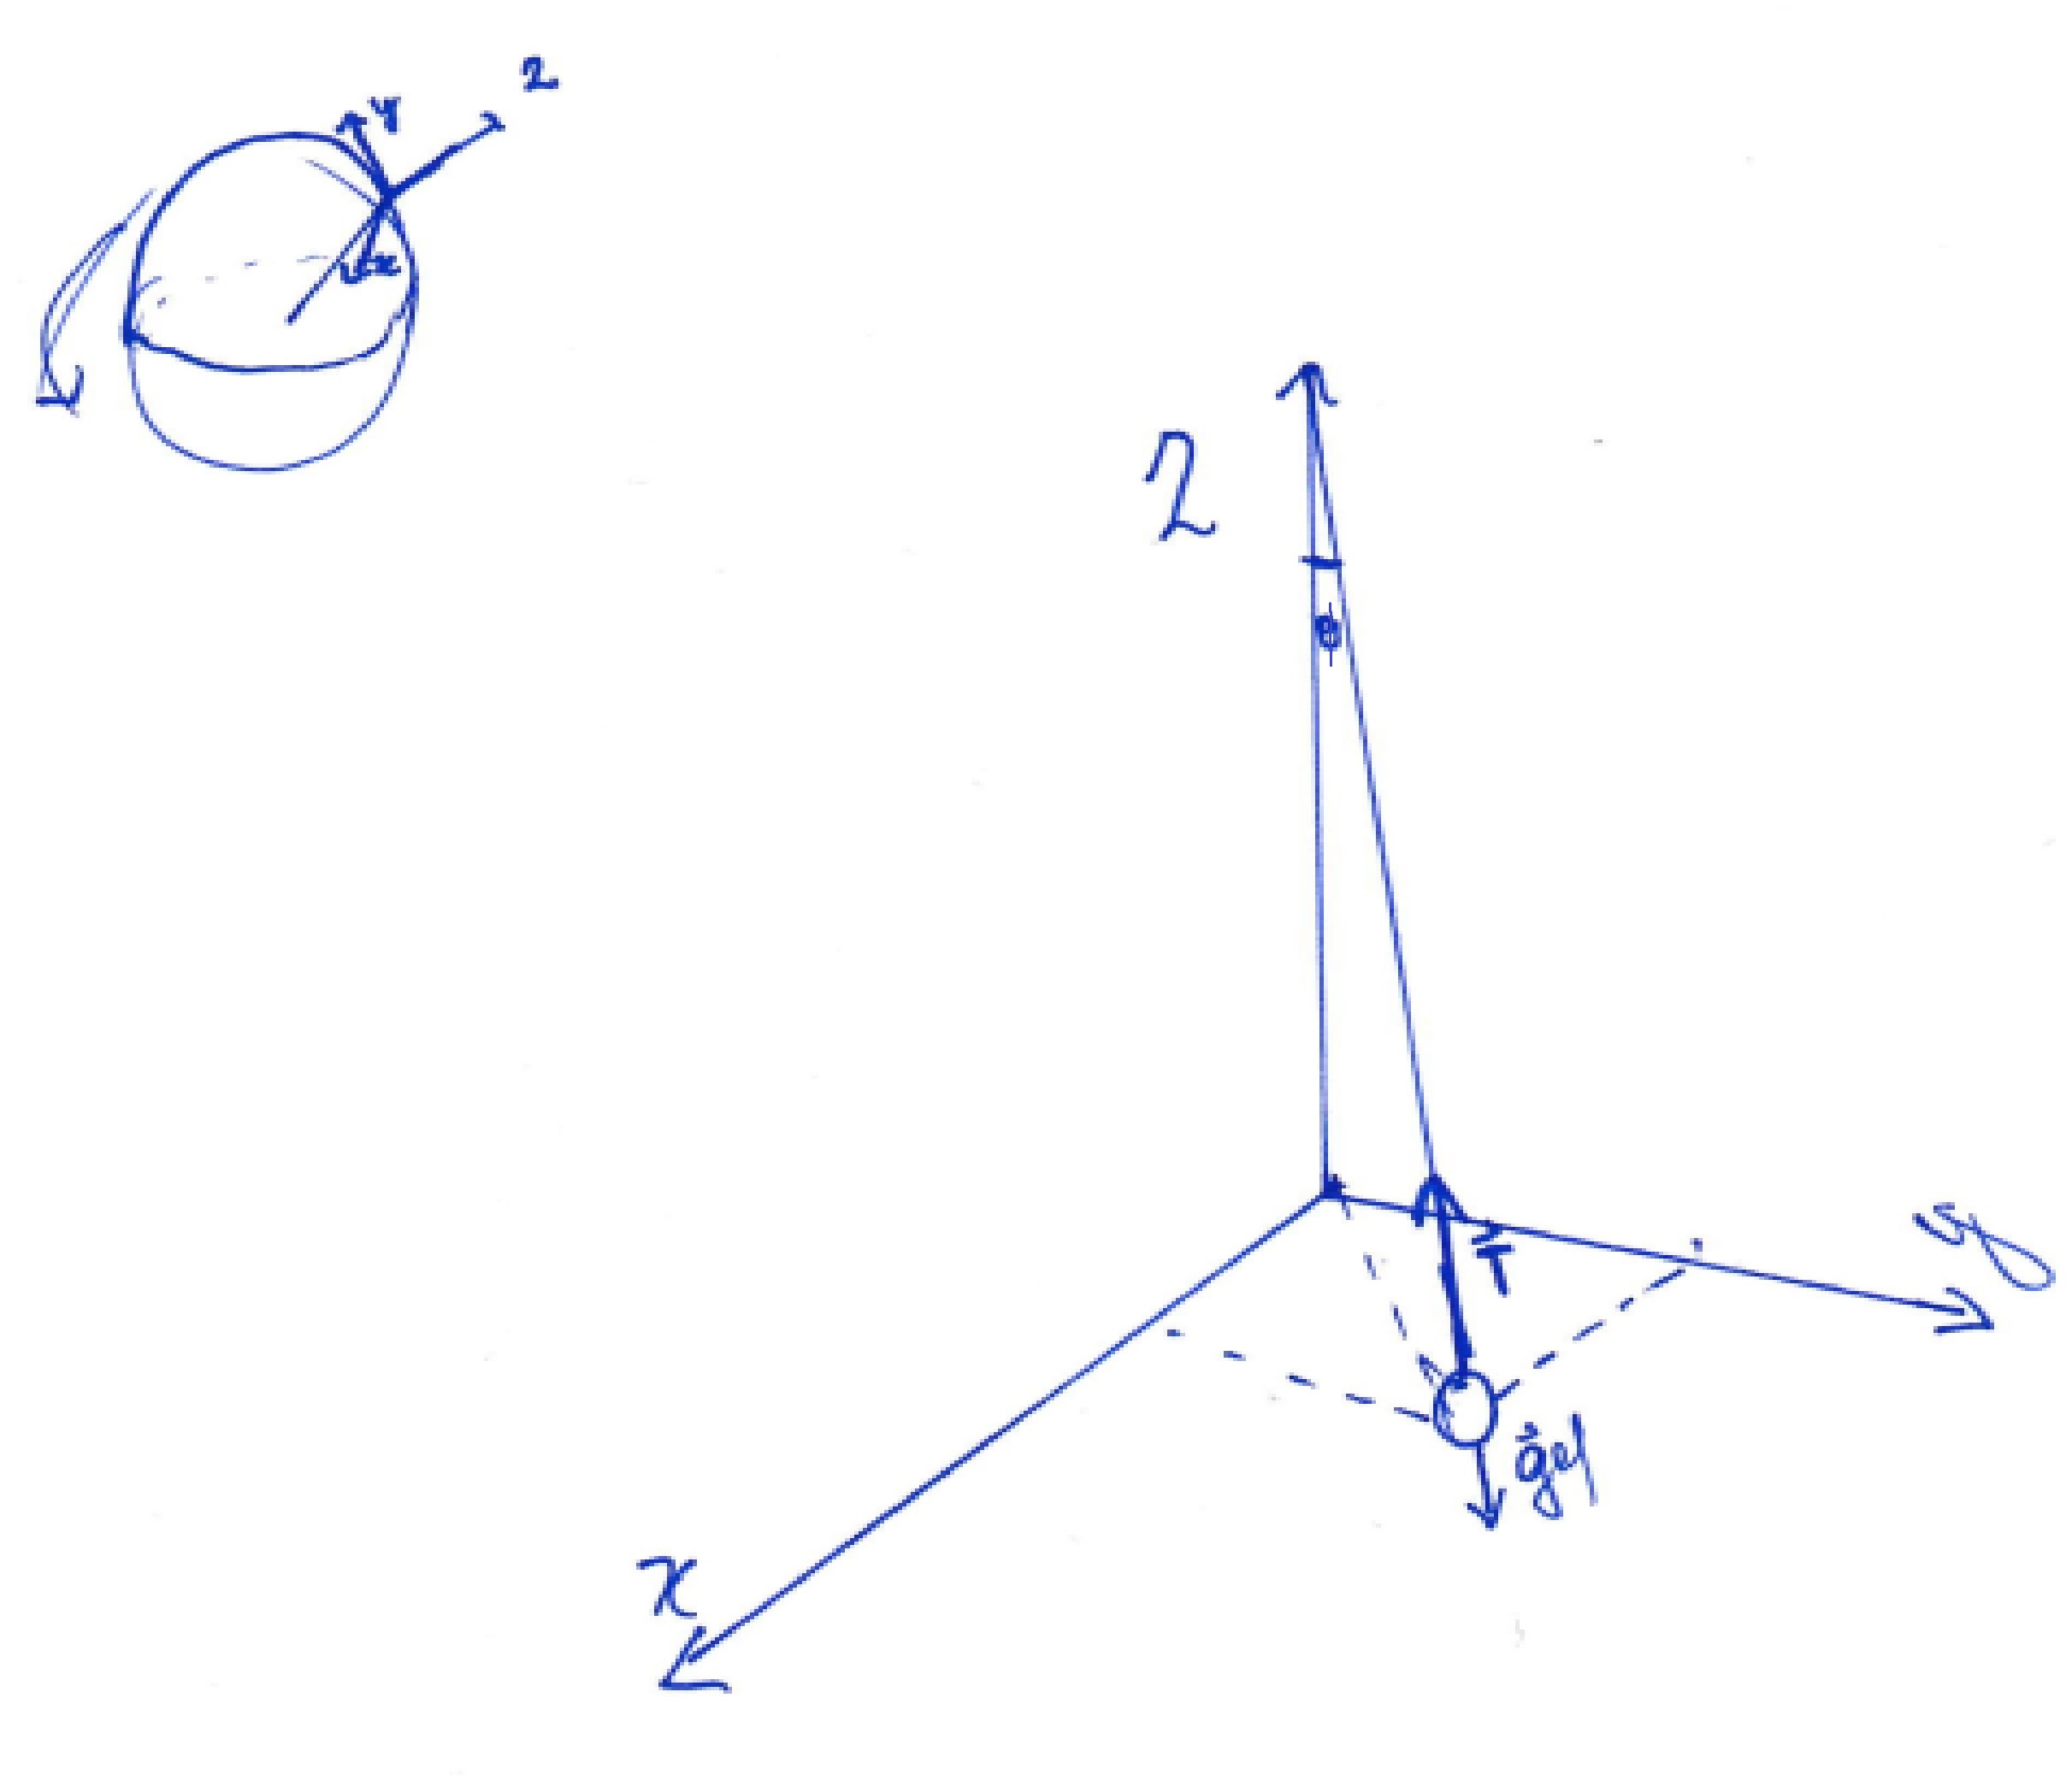
\includegraphics[width=0.5\textwidth]{foucault.jpg}
  \caption{Representación del problema}
  \label{fucas}
\end{figure}


Como estamos en el sistema de la Tierra, sabemos que podemos escribir la segunda Ley de Newton para este sistema como:

\begin{equation}
  m\ddot{\boldsymbol{r}} = \boldsymbol{F}_{ap} + \boldsymbol{F}_{cf} + \boldsymbol{F}_{cor}
\end{equation}

Para nuestro problema en particular, la fuerza aplicada será, por un lado, la tensión y, por otro, la gravedad. De esta manera, tendremos que:

\begin{equation}
  m \ddot{\boldsymbol{r}} = \boldsymbol{T} + m\boldsymbol{g} + m(\boldsymbol{\Omega} \times \boldsymbol{r}) + 2m (\dot{\boldsymbol{r}} \times \boldsymbol{\Omega})
\end{equation}

Esta ecuación se puede simplificar bastante si consideramos que el término centrífugo se puede combinar al gravitatorio y, al final, tendremos un término de la gravedad efectiva\footnote{Tomaremos esto simplemente como un hecho conocido, pero cualquier libro texto estándar de mecánica lo tiene tratado explícitamente.}:

\begin{equation}
  \label{initialus1}
  m \ddot{\boldsymbol{r}} = \boldsymbol{T} + m\boldsymbol{g}_ef + 2m (\dot{\boldsymbol{r}} \times \boldsymbol{\Omega})
\end{equation}

Para proseguir en la resolución, tendremos que mirar el problema en concreto. Primeramente, podemos escribir que, en el eje $z$, la segunda ley de Newton tendrá forma aproximadamente\footnote{Aquí estamos aproximando la fuerza de Coriolis no tiene efecto en el eje $z$ y que partícula aproximadamente no se mueve   } 

$$T_{z} - mg_{ef} \approx 0$$

Por la figura \ref{fucas}, sabemos por trigonometría básica que $T_{z} = T \cos{\phi}$. Como estamos en el régimen de oscilaciones pequeñas en $\phi$, sabemos que:

\begin{equation}
  T_{z} \approx T
\end{equation}

Si juntamos las dos condiciones, tendremos que:

\begin{equation}
  T \approx m g_ef 
\end{equation}

Como queríamos demostrar.

\subsection*{b) Escriba las ecuaciones de movimiento del plano horizontal en forma matricial}

Como asumimos en nuestra aproximación que no había movimiento vertical, nos resta analizar el movimiento horizontal. Inicialmente, escribimos en coordenadas el término de Coriolis. Como $\dot{\boldsymbol{r}} = (\dot{x},\dot{y},\dot{z})$ y $\boldsymbol{\Omega} = (0,\Omega \sin\theta, \Omega \cos\theta)$:

$$\boldsymbol{F}_{cor} = 2m (\dot{\boldsymbol{r}} \times \boldsymbol{\Omega}) = 2 m (\dot{y}\Omega \cos\theta-\dot{z} \sin\theta, -\dot{x}\Omega \cos\theta, \dot{x} \Omega \sin\theta )$$

Como ya lo decimos, vamos a ignorar el término vertical en este problema, entonces tomaremos el término de Coriolis como $\boldsymbol{F}_{cor}= 2 m (\dot{y}\Omega \cos\theta, -\dot{x}\Omega \cos\theta )$. Por la ecuación \eqref{initialus1}, si determinamos las tensiones determinaremos las ecuaciones de movimiento. Eso se puede hacer de manera casi trivial con un poco de trigonometría, de la que concluiremos que $\frac{T_x}{T} = -\frac{x}{\ell} $ y $\frac{T_y}{T} = -\frac{y}{\ell}$\footnote{El signo negativo es una sutileza que se puede fácilmente olvidar, pero viene del hecho de que la tensión estará siempre opuesta al movimiento. Si no lo fuera, la solución explotaría y eso claramente no es una solución física para un péndulo.}. De eso, concluimos que:
$$T_x = -\frac{mgx}{\ell} $$
$$T_y = -\frac{mgy}{\ell} $$

De manera que podemos escribir las ecuaciones de movimiento:
\begin{equation}
  \begin{aligned}
    \ddot{x} = -\frac{g x}{\ell} + 2\dot{y}\Omega \cos\theta\\
    \ddot{y} = -\frac{g y}{\ell} - 2\dot{x}\Omega \cos\theta
  \end{aligned}
\end{equation}

O sea, lo escribimos aqui como:

\begin{equation}
  \begin{aligned}
    \label{eqmov1}
    \ddot{x} - 2\dot{y}\Omega \cos\theta + \frac{g x}{\ell} = 0\\
    \ddot{y}  + 2\dot{x}\Omega \cos\theta + \frac{g y}{\ell} = 0
  \end{aligned}
\end{equation}

Que podemos escribir vectorialmente como:

\begin{equation}
  \ddot{\boldsymbol{\chi}} +A\dot{\chi} + B \boldsymbol{\chi} = 0
\end{equation}

Donde:
\begin{equation}
  \boldsymbol{\chi} = \begin{pmatrix} x \\ y\end{pmatrix} \qquad 
  A = 2\Omega \cos\theta \begin{pmatrix} 0 & -1 \\ 1 & 0\end{pmatrix} \qquad
  B = \frac{g}{\ell} \begin{pmatrix} 1 & 0 \\ 0 & 1\end{pmatrix}
\end{equation}

Que era lo que queríamos encontrar.

\subsection*{c) Integre las ecuaciones de movimiento de manera exacta y demuestra que la órbita del grave es una elipse que precesa con velocidad angular $\Omega \cos\theta$.}

Para integrar nuestra ecuación, utilizaremos la técnica que vimos en clases de introducir una variable  compleja\footnote{Más que una coincidencia feliz, es casi siempre ideal introducir números complejos para tratar de rotaciones en $\mathbb{R}^{2}$ , que es exactamente la esencia de nuestro problema, por el isomorfismo entre $SO(2)$ y $U(1)$.} , $z = x + i y $. Si sumamos la primera fila por $i$ veces la segunda. Lo hacemos explícitamente:

$$\ddot{x} + i\ddot{y} + 2\Omega \cos\theta(\dot{y} -i \dot{x}) + \frac{g}{\ell} (x + i y) =\frac{d^2}{dt^2} \left(x + i y\right) + 2\Omega \cos\theta\frac{d}{dt}-i (iy + x) + \frac{g}{\ell} (x + i y) = 0 $$

$$\ddot{z} - 2i\Omega\cos\theta \dot{z} + \frac{g}{\ell} z = 0$$

Para encontrar la solución de este sistema lineal de orden dos, probaremos una solución de tipo $z(t) = e{i\lambda t}$:

$$e^{i\lambda t} (-\lambda^2 - 2\Omega \cos{\theta} \lambda + \frac{g}{l}) = 0$$

De manera que tendremos dos valores de lambda como solución:

$$\lambda = \Omega \cos\theta \pm \sqrt{(\Omega\cos\theta)^2 + \left(\frac{g}{l}\right)^2} = \Omega_\theta \pm \omega$$

Donde, por claridad, hemos definido $\Omega_\theta = \Omega \cos\theta$ y $\omega = \sqrt{(\Omega\cos\theta)^2 + \left(\frac{g}{l}\right)^2}$. De esa manera, tendremos que la solución general para nuestro problema será:

$$z = C_1 e^{it(\Omega + \omega)} +C_2 e^{it(\Omega - \omega)} = C_1 e^{i\Omega t} e^{i\omega t} + C_2 e^{i \Omega t} e^{-i\omega t} = e^{i\Omega t}\left(C_1 e^{i\omega t} + C_2 e^{-i\omega t}\right) $$

\begin{equation}
  \label{sol1}
  z = e^{i\Omega t}\left(C_1 e^{i\omega t} + C_2 e^{-i\omega t}\right) 
\end{equation}

Si queremos explícitamente encontrar las soluciones en nuestras variables original, sabemos que $x = \Re (z)$ e $y = \Im (z)$ y estas son operaciones triviales de hacer, pero no iluminan mucho nuestra solución.\footnote{Hacer eso sería como resolver el problema de dos cuerpos en polares y pasarlo a cartesianas para `interpretar los resultados'}. Si miramos directamente a la ecuación \eqref{sol1}, podremos apreciar que tenemos un término envolvente, de frecuencia $\Omega_{\theta}$, y otro término interior, combinación lineal de frecuencias $\omega$ y $-\omega$. Este término interior corresponde exactamente a una elipsis en el plano complejo, y el exterior a una rotación de esta elipsis (Esto es, un término de precesión). Para valores escogidos de manera aleatoria, tenemos la siguiente representación gráfica:

\begin{figure}
  \centering
  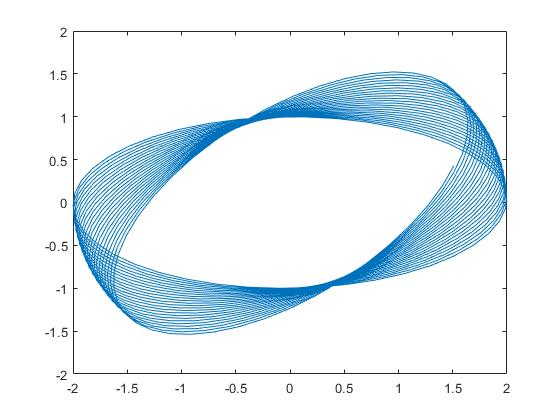
\includegraphics[width=\textwidth]{foucgraph.jpg}
  \caption{Gráfico de los 15 primeros segundos para $C_1 = C_2 + 1 = 1.5 $, $\Omega_\theta = 0.05 Hz$ y $\omega = 10 Hz$}
\end{figure}

De esa manera, encontramos la solución exacta para nuestra ecuación diferencial y demostramos que es una elipsis que precesa con velocidad angular $\Omega_\theta = \Omega \cos\theta$, que es exactamente lo que se pedía.

\subsection*{d) Integra la ecuación diferencial del apartado anterior de manera perturbativa hasta primer orden en $\Omega$}

\subsubsection*{Solución de Orden 0}
El método perturbativo siempre empieza por la solución de orden 0, esto es, donde no consideramos los términos con $\Omega$\footnote{Formalmente, asumimos que la solución va con potencias de $\Omega$ y agrupamos términos del mismo orden.}. De las ecuaciones\eqref{eqmov1} y tomando $\omega_{0}^2 = \frac{g}{\ell} $, tenemos que:

\begin{equation}
  \label{0th}
  \begin{aligned}
  \ddot{x}_0 + \omega_0^2 x_0 = 0\\
  \ddot{y}_0 + \omega_0^2 y_0 = 0
\end{aligned}
\end{equation}

Que son absolutamente triviales de resolver, ya que son apenas osciladores armónicos desacoplados:

\begin{equation}
\begin{aligned}
  x_0(t) = A_1 \cos(\omega_0 t + \delta_1)\\
  y_0(t) = A_2 \cos(\omega_0 t + \delta_2) 
\end{aligned}
\end{equation}

\subsubsection{Solución de Orden 1}
Finalmente, podemos poner los términos que van en orden 1:

\begin{equation*}
\begin{aligned}
  \ddot{x}_1 - 2 \dot{y}_0 + \omega_0^2 x_1 = 0\\
  \ddot{y}_1 + 2 \dot{x}_0 + \omega_1^2 y_1 = 0
\end{aligned}
\end{equation*}

Que podemos escribir como:

\begin{equation}
\begin{aligned}
  \ddot{x}_1 + \omega_0^2 x_1 = -2A_2 \omega_0 \sin(\omega_0 t + \delta_2)\\
  \ddot{y}_1 + \omega_0^2 y_1 = 2A_1 \omega_0 \sin(\omega_0 t + \delta_1)
\end{aligned}
  \label{1st}
\end{equation}

\subsection*{e) Demuestra que el período de oscilación del péndulo es aproximadamente $T = T_{0}(1-\frac{\Omega^2}{2\omega^2_0}\cos^2\theta) $}

En la sección c), determinamos que el péndulo oscilaba con frecuencia angular $\omega = \sqrt{(\Omega\cos\theta)^2 + \left(\frac{g}{l}\right)^2}$. Podemos manipular un poco esta expresión:

$$\omega =\sqrt{(\Omega\cos\theta)^2 + \omega_0^2} = \omega_0 \sqrt{1 + \frac{\Omega^2}{\omega_0^2} \cos^2\theta} $$

Por definición, sabemos que el período está relacionado con la frecuencia angular por:

$$T = \frac{2\pi}{ \omega}$$

De manera que, para nuestra frecuencia particular tendremos que:

$$T = \frac{2\pi}{\omega_0} \left(1 + \frac{\Omega^2}{\omega_0^2}\right)^{-\frac{1}{2}}$$

Pero, sabemos que $T_{0} =\frac{2\pi}{\omega} $ y que podemos aproximar $(1+x)^{n} =1+nx$, o sea, podemos escribir que:

\begin{equation}
  T \approx \frac{2\pi}{\omega_0} \left(1 - \frac{\Omega^2}{2\omega^2}\right)
\end{equation}

Que era lo que queríamos demostrar.

\subsection*{f) Calcula el tiempo que tarda el péndulo en dar una vuelta completa alrededor de su eje de giro y estima dicho tiempo para la facultad}

Sabemos que la frecuencia angular de precesión del péndulo es $\Omega_{\theta} = \Omega \cos\theta$, y que está frecuencia angular está relacionada con el período por:

$$T_{prec} = \frac{2\pi}{\Omega_\theta} = \frac{2\pi}{\Omega} \sec\theta = T_{tierra} \sec\theta $$

Finalmente, sabemos que Salamanca está a una colatitud de $\theta = 49.03118°$ y que el periodo de la tierra es de 24h, y por lo tanto sabemos que

$$T_{precUSAL} = 36.60 h = 36h 36 min$$

\section{ Cánica puntual sobre cara interna de un cono hueco}

\subsection*{a) Calcula el momento de inercia del cono alrededor de su eje de giro y escribe el Lagrangeano del sistema cánica + cono en un sistema inercial.}

Para calcular el momento de inercia del cono, utilizaremos que:

$$I = \int r^2 dm = \int_S \sigma r^2  d\Omega$$

Pero sabemos que podemos parametrizar (en cartesianas) el cono como: $(z \tan\alpha \cos\theta, z \tan\alpha \sin\theta, z)$. Calculamos los vectores tangentes:
$$\boldsymbol{v}_\theta = z (-\tan\alpha \sin\theta,\tan\alpha \cos\theta , 0)$$
$$\boldsymbol{v}_z = (\tan\alpha\cos\theta,\tan\alpha\sin\theta,1)$$

De manera que:
$$||\bolsymbol{n}|| = z\tan\alpha\sec{\alpha}$$

$$I= \sigma \int r^2 ||n||dzd\phi = \sigma\int_0^{2\pi}d\theta z^3 \tan\alpha \sec^3\alpha \int_0^h    dz = \sigma 2\pi \frac{h^4}{4} \tan\alpha \sec^3\alpha$$

$$I = \sigma \pi (h\sec\alpha)^2 $$

Para el lagrangeano, tendremos 3 términos cinéticos y 2 potenciales: 2 cinéticos para el cono (uno de rotación y otro de traslación) y uno para la masa, y un potencial para cada. Escribiéndolo, tenemos que:

$$T = T_{rot} + T_{trans} + T_{cuenca} = \frac{1}{2} I \omega^2(t) + \frac{1}{2} M \dot{Z} + \frac{1}{2} m  (\dot{r}^2 + r^2 \dot{\phi}^2+\dot{z}^2)$$

$$V = M g Z + mgz$$

Finalmente, 

\begin{equation}
  \mathcal{L} = \frac{1}{2} I \omega^2(t) + \frac{1}{2} M \dot{Z}^2 + \frac{1}{2} m  (\dot{r}^2 + r^2 \dot{\phi}^2+\dot{z}^2) - M g Z - mgz
\end{equation}



\end{document}

